\begin{figure}%[!htb] 
\centering 
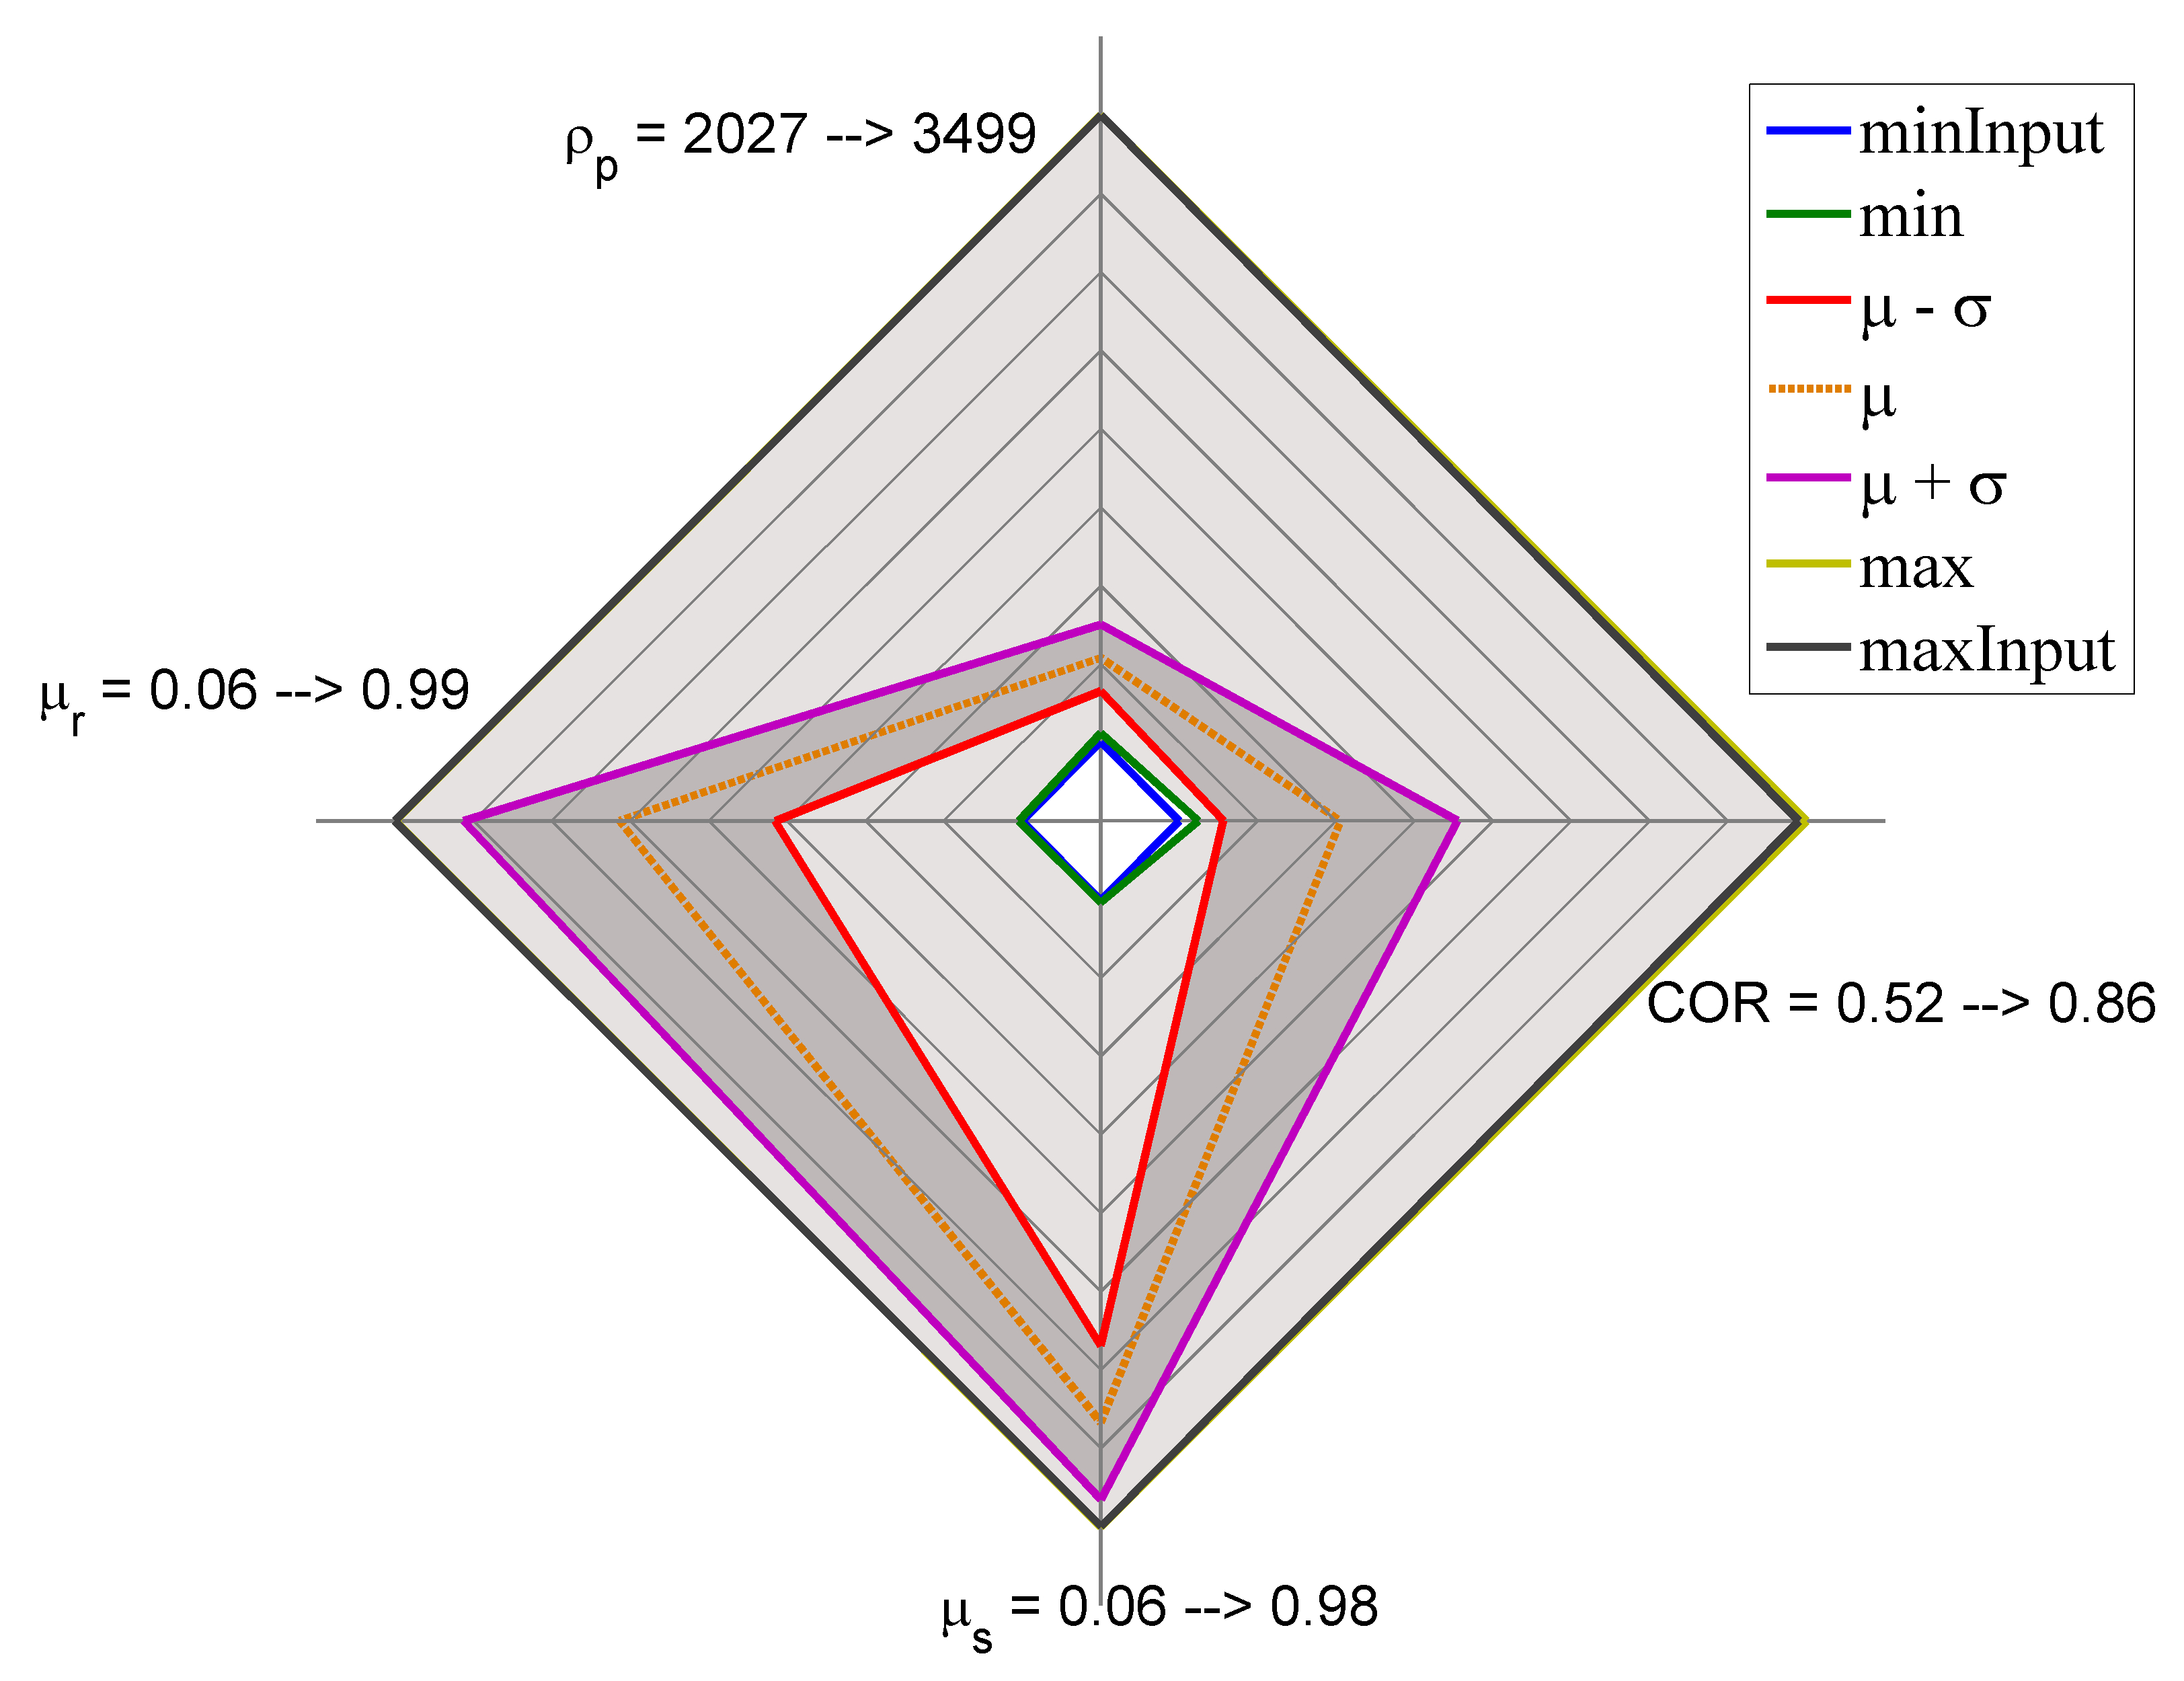
\includegraphics[width=.48\columnwidth]{images/26radarpirker08schulze10070} 
\caption{Parameter space plot, $SSC$, $\sigma_n=10070$ Pa, P=0.8}
\label{fig:26radarpirker08schulze10070} 
\end{figure}
%************************************************
\begin{figure}%[!htb] 
\centering 
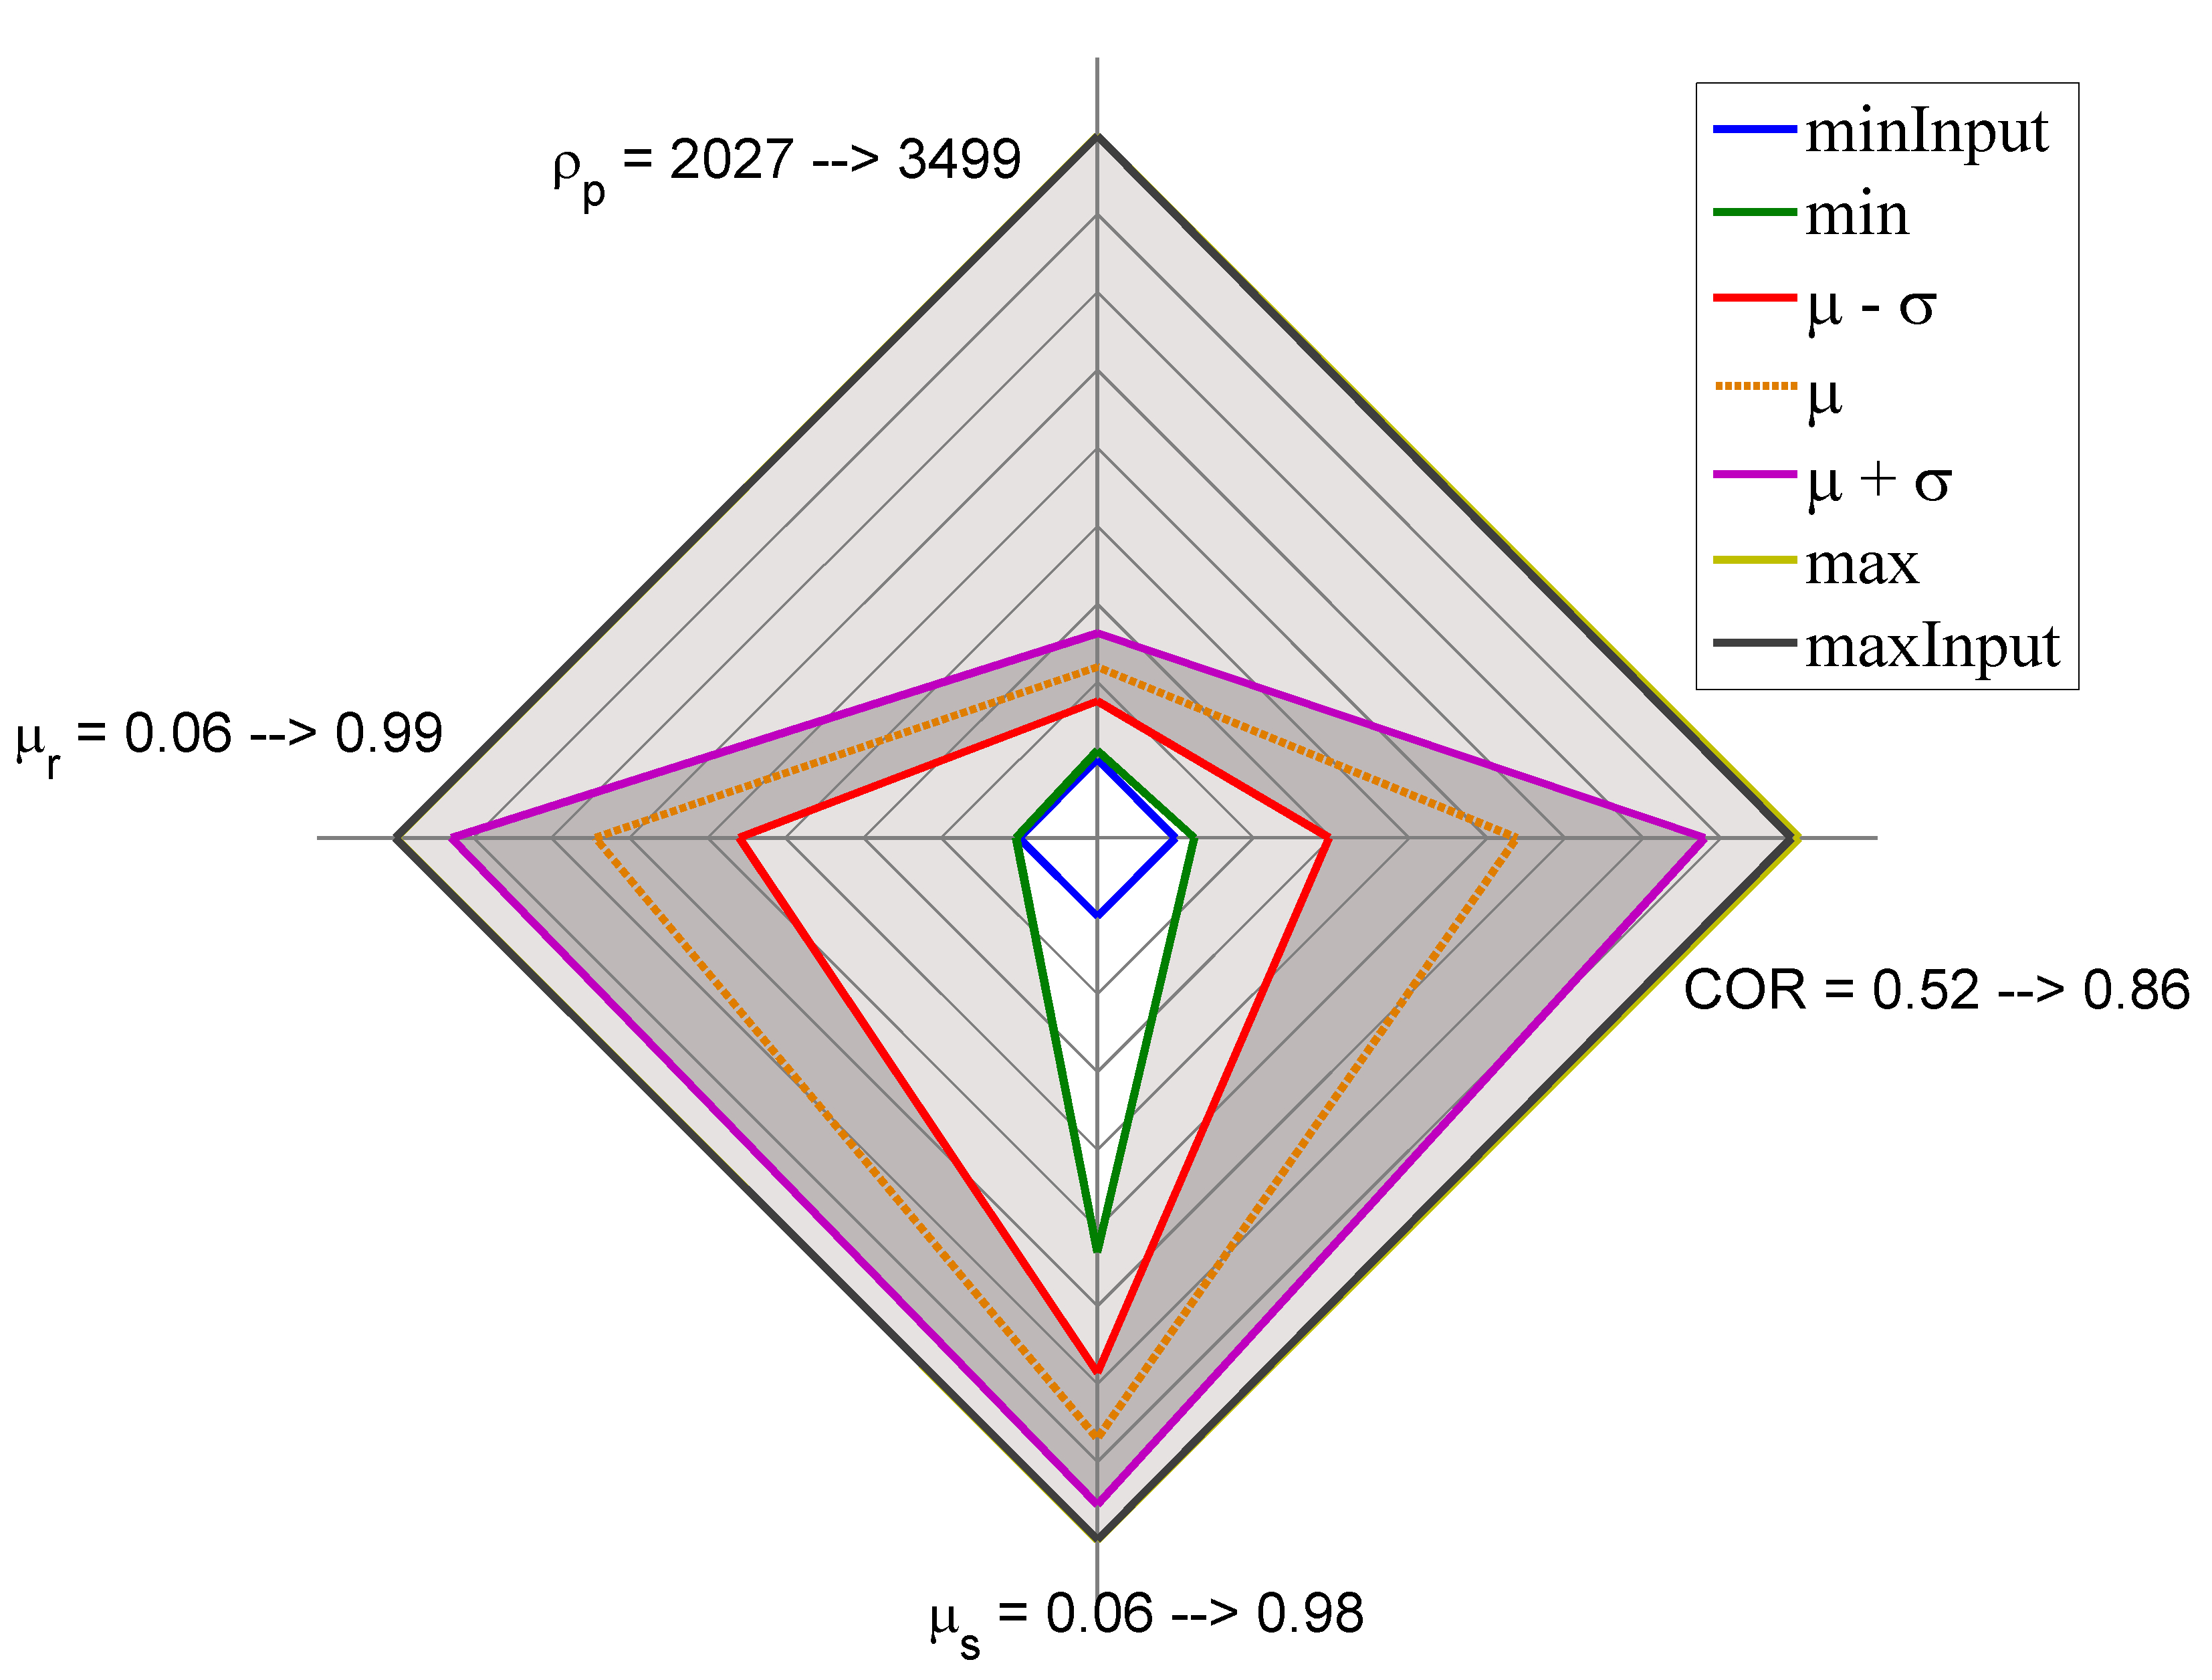
\includegraphics[width=.48\columnwidth]{images/24radarpirker1schulze10070} 
\caption{Parameter space plot, $SSC$, $\sigma_n=10070$ Pa, P=1.0}
\label{fig:24radarpirker1schulze10070} 
\end{figure}
%************************************************
\begin{figure}%[!htb] 
\centering 
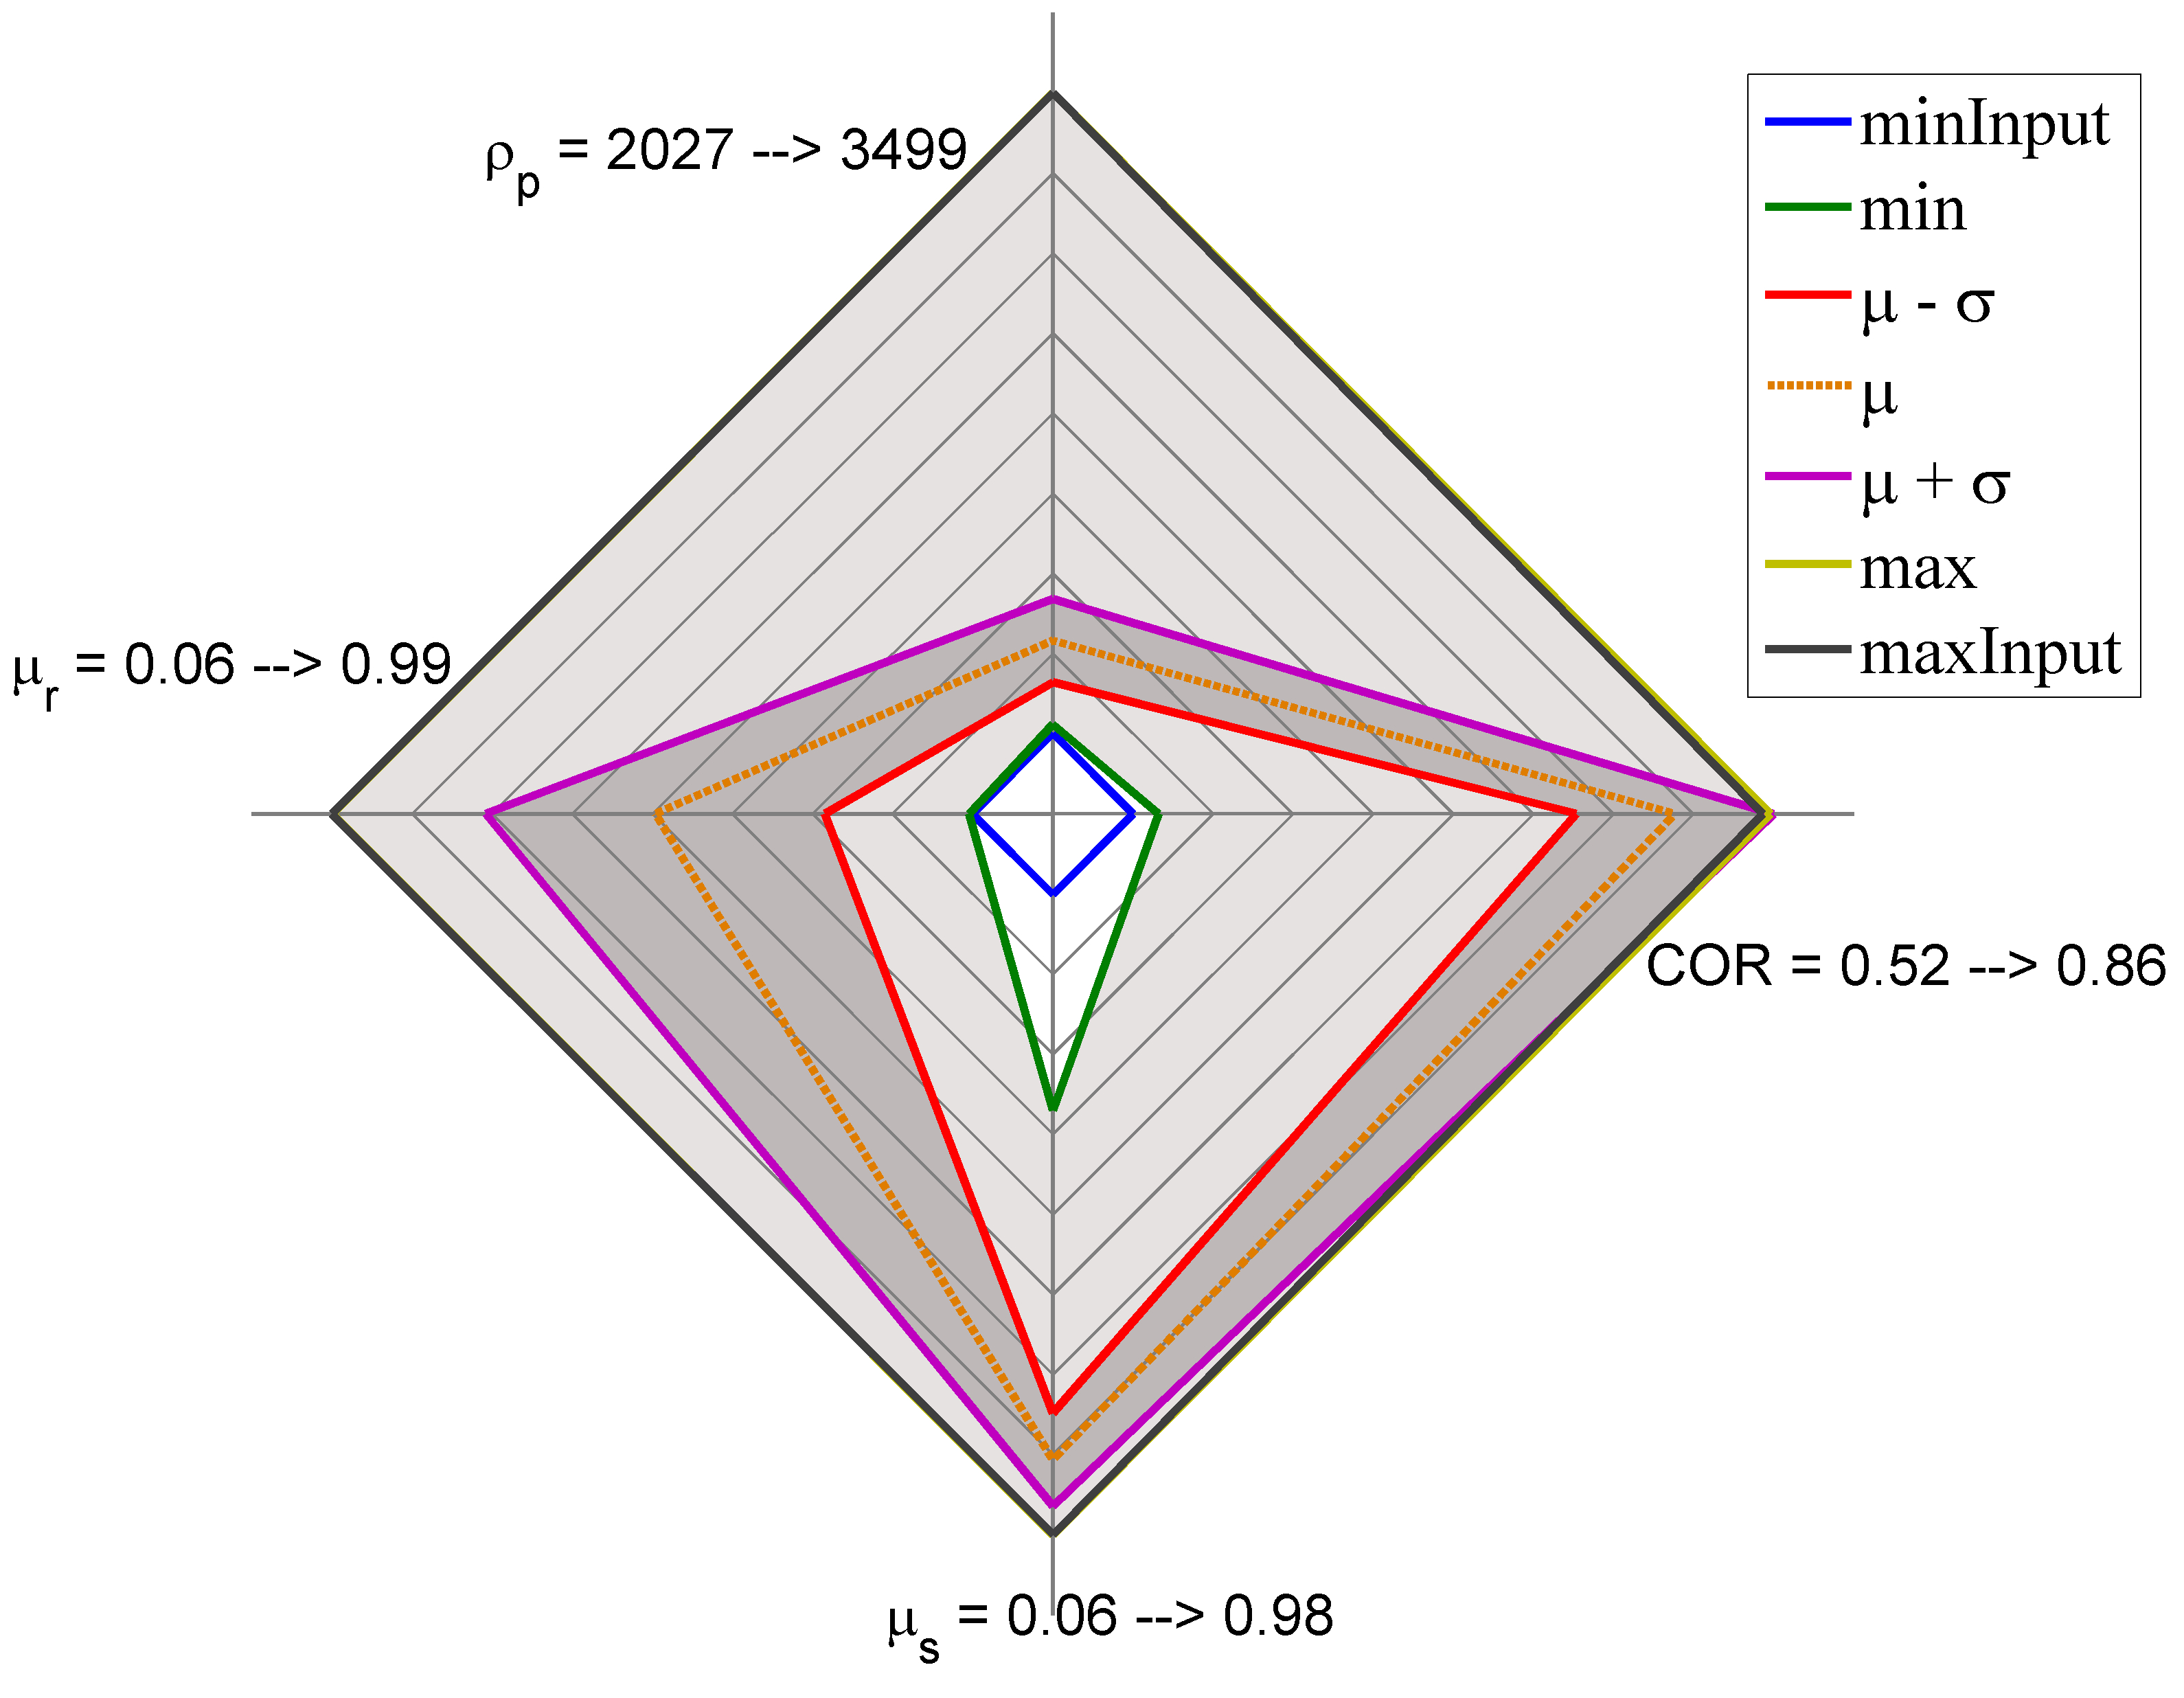
\includegraphics[width=.48\columnwidth]{images/28radarpirker12schulze10070} 
\caption{Parameter space plot, $SSC$, $\sigma_n=10070$ Pa, P=1.2}
\label{fig:28radarpirker12schulze10070} 
\end{figure}
%************************************************
\begin{figure}%[!htb] 
\centering 
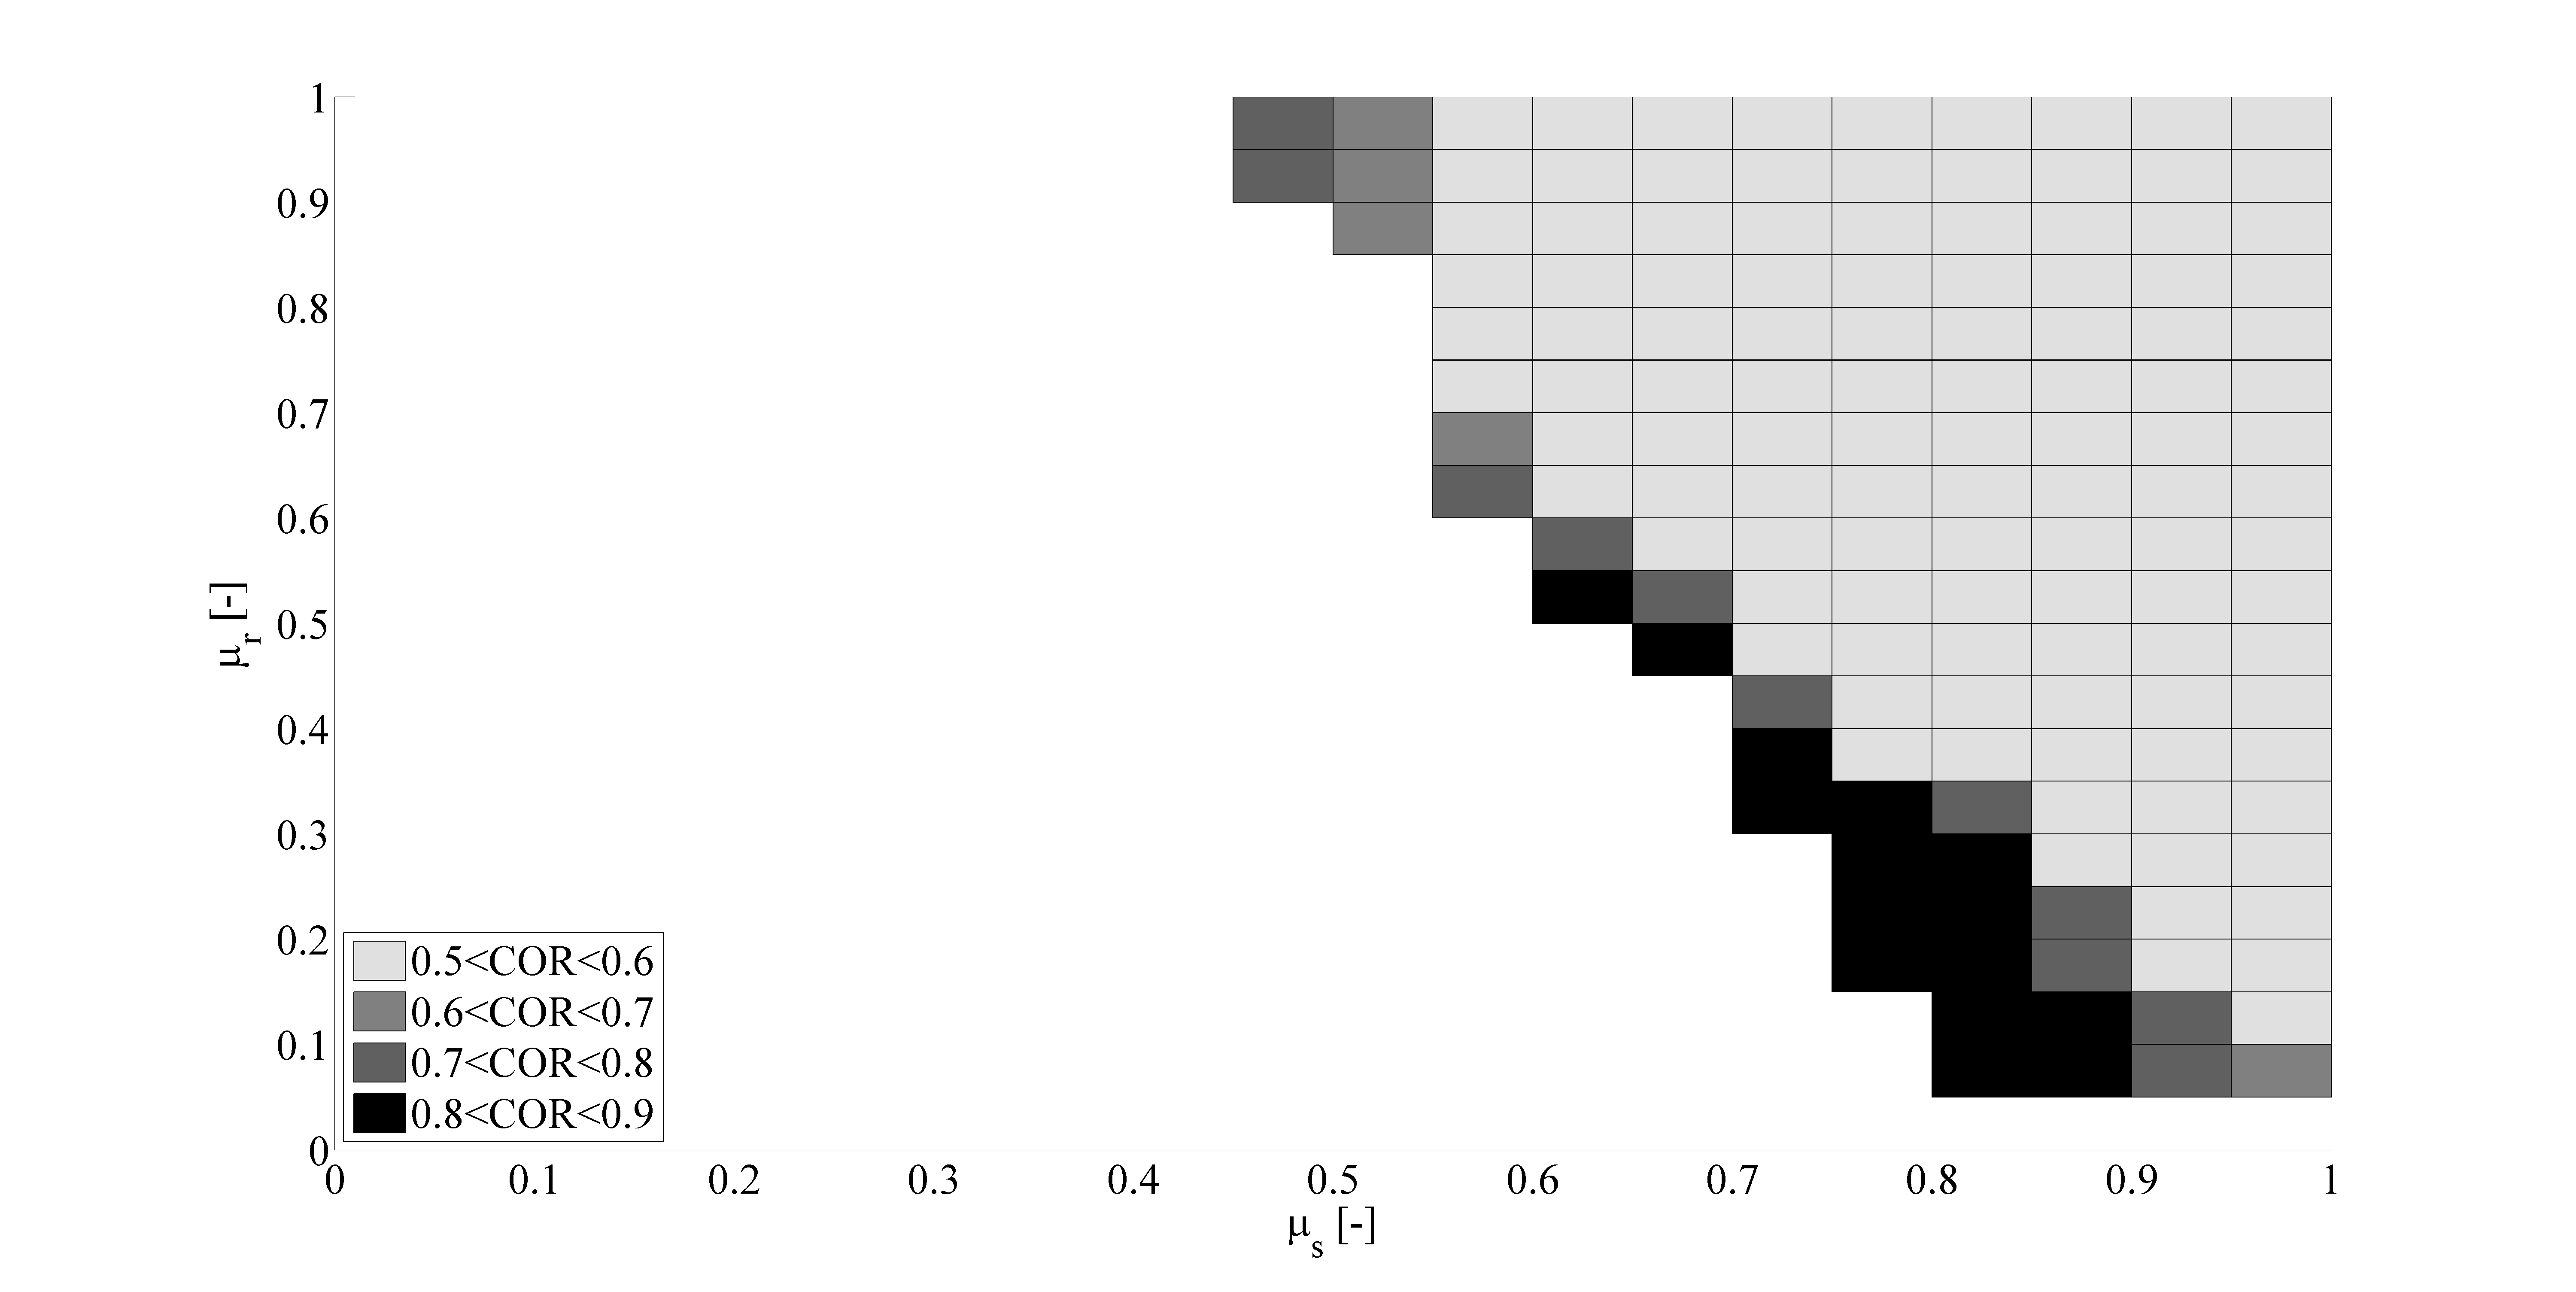
\includegraphics[width=.48\columnwidth]{images/27cloudpirker08schulze10070} 
\caption{Density plot, $SSC$, $\sigma_n=10070$ Pa, P=0.8}
\label{fig:27cloudpirker08schulze10070} 
\end{figure}
%************************************************
\begin{figure}%[!htb] 
\centering 
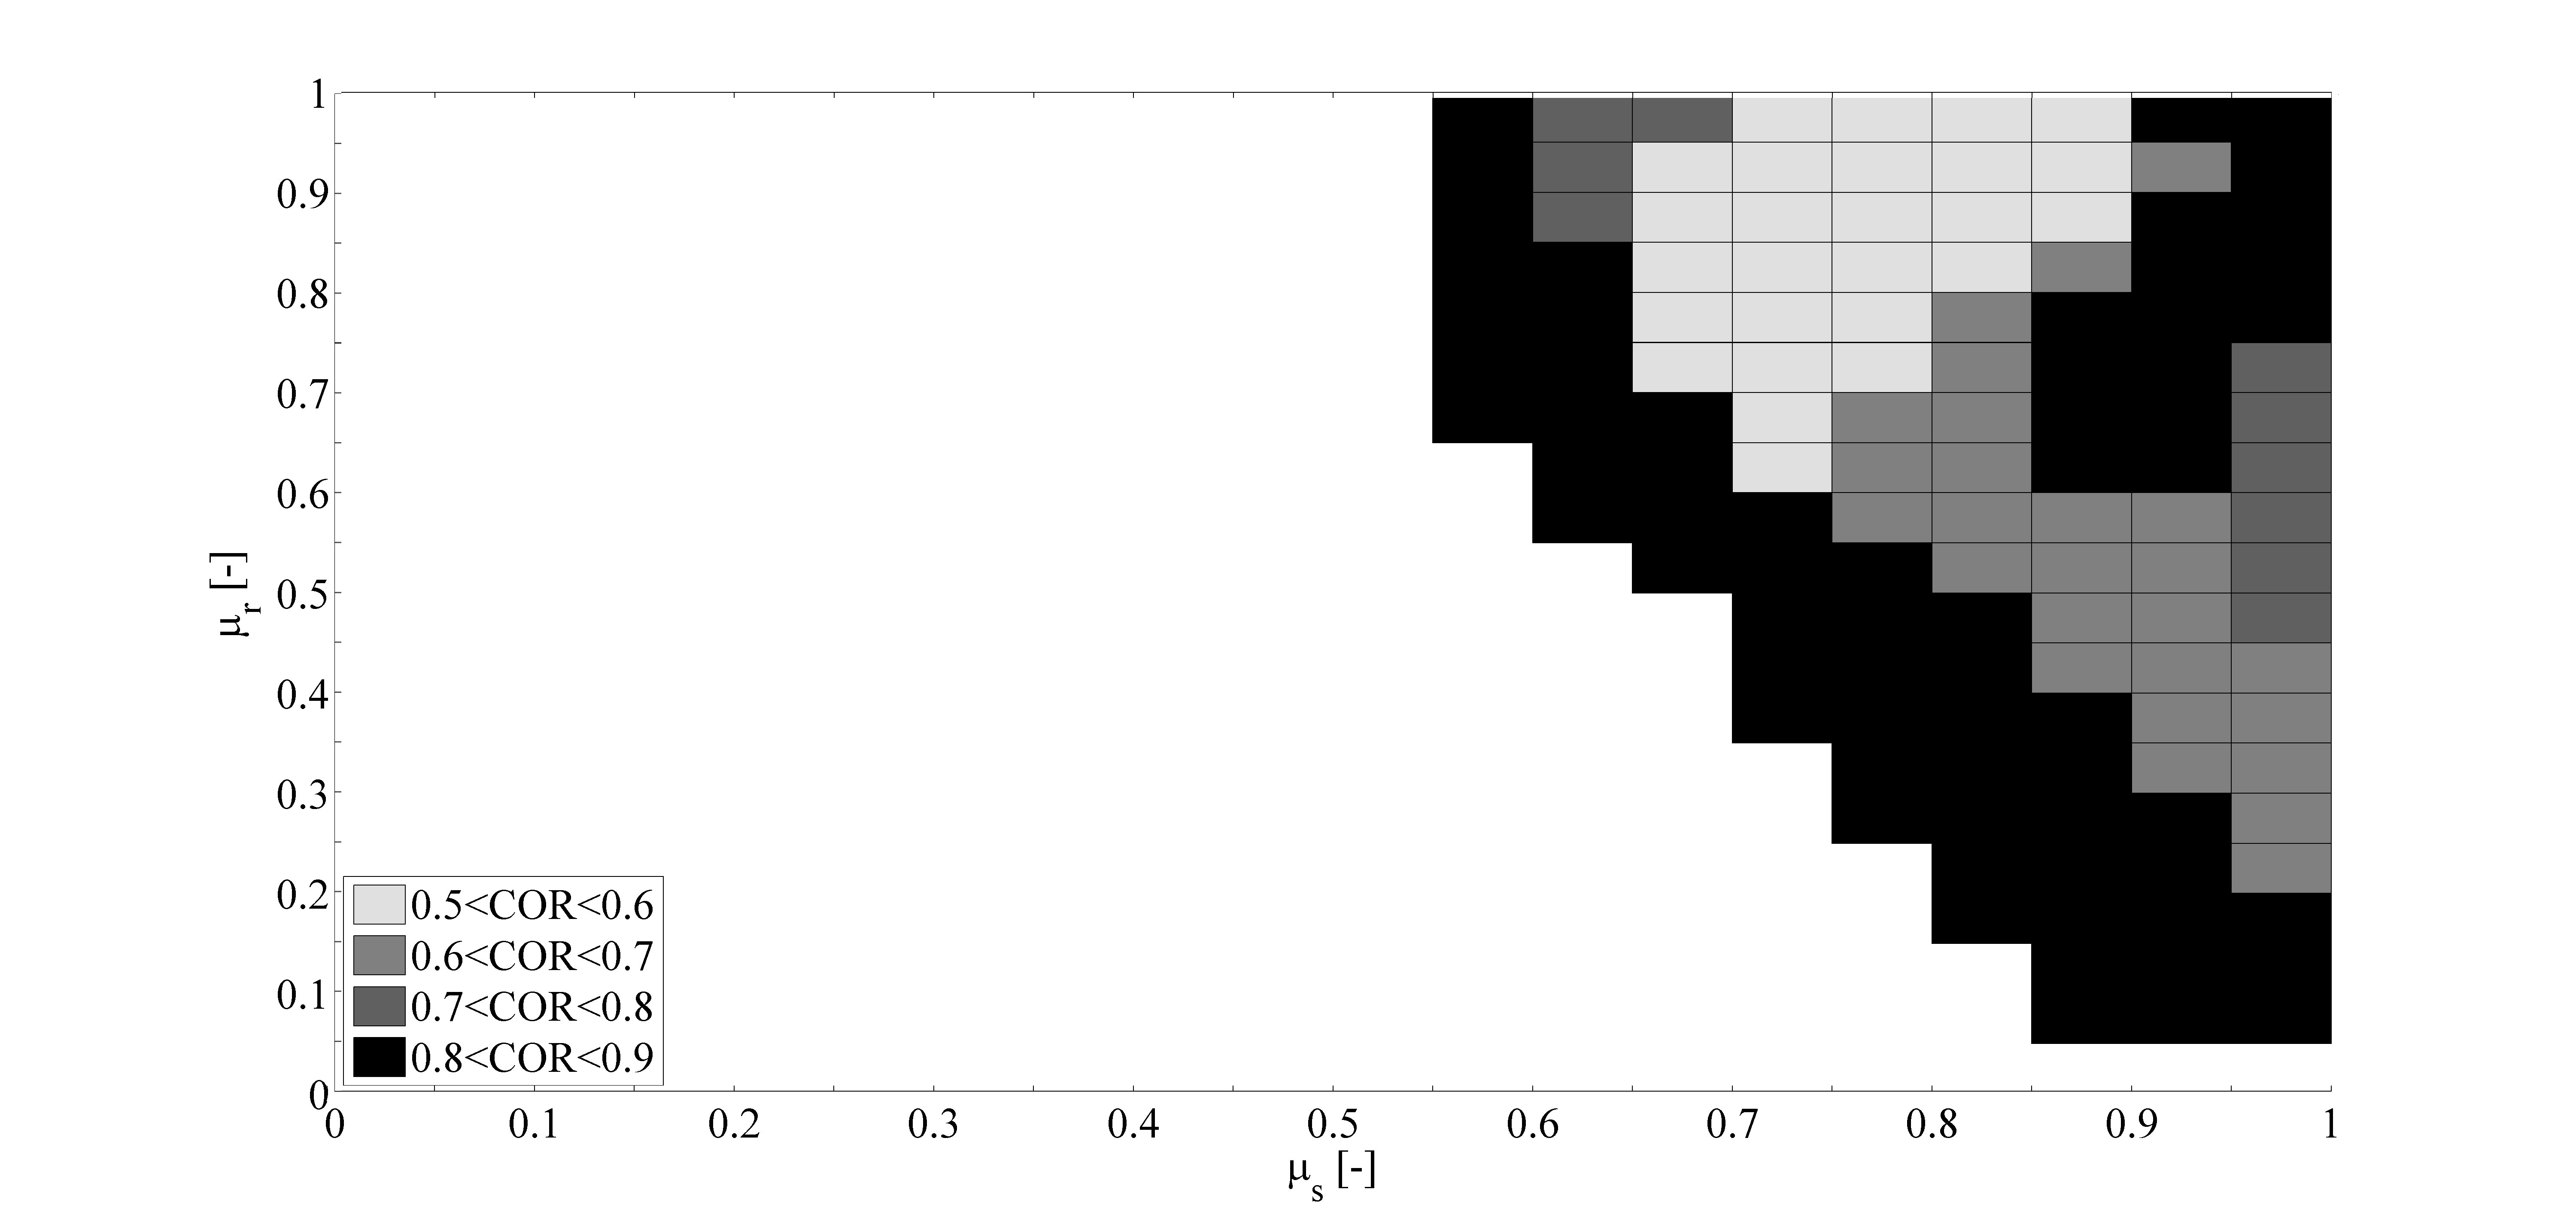
\includegraphics[width=.48\columnwidth]{images/25cloudpirker1schulze10070} 
\caption{Density plot, $SSC$, $\sigma_n=10070$ Pa, P=1.0}
\label{fig:25cloudpirker1schulze10070} 
\end{figure}
%************************************************
\begin{figure}%[!htb] 
\centering 
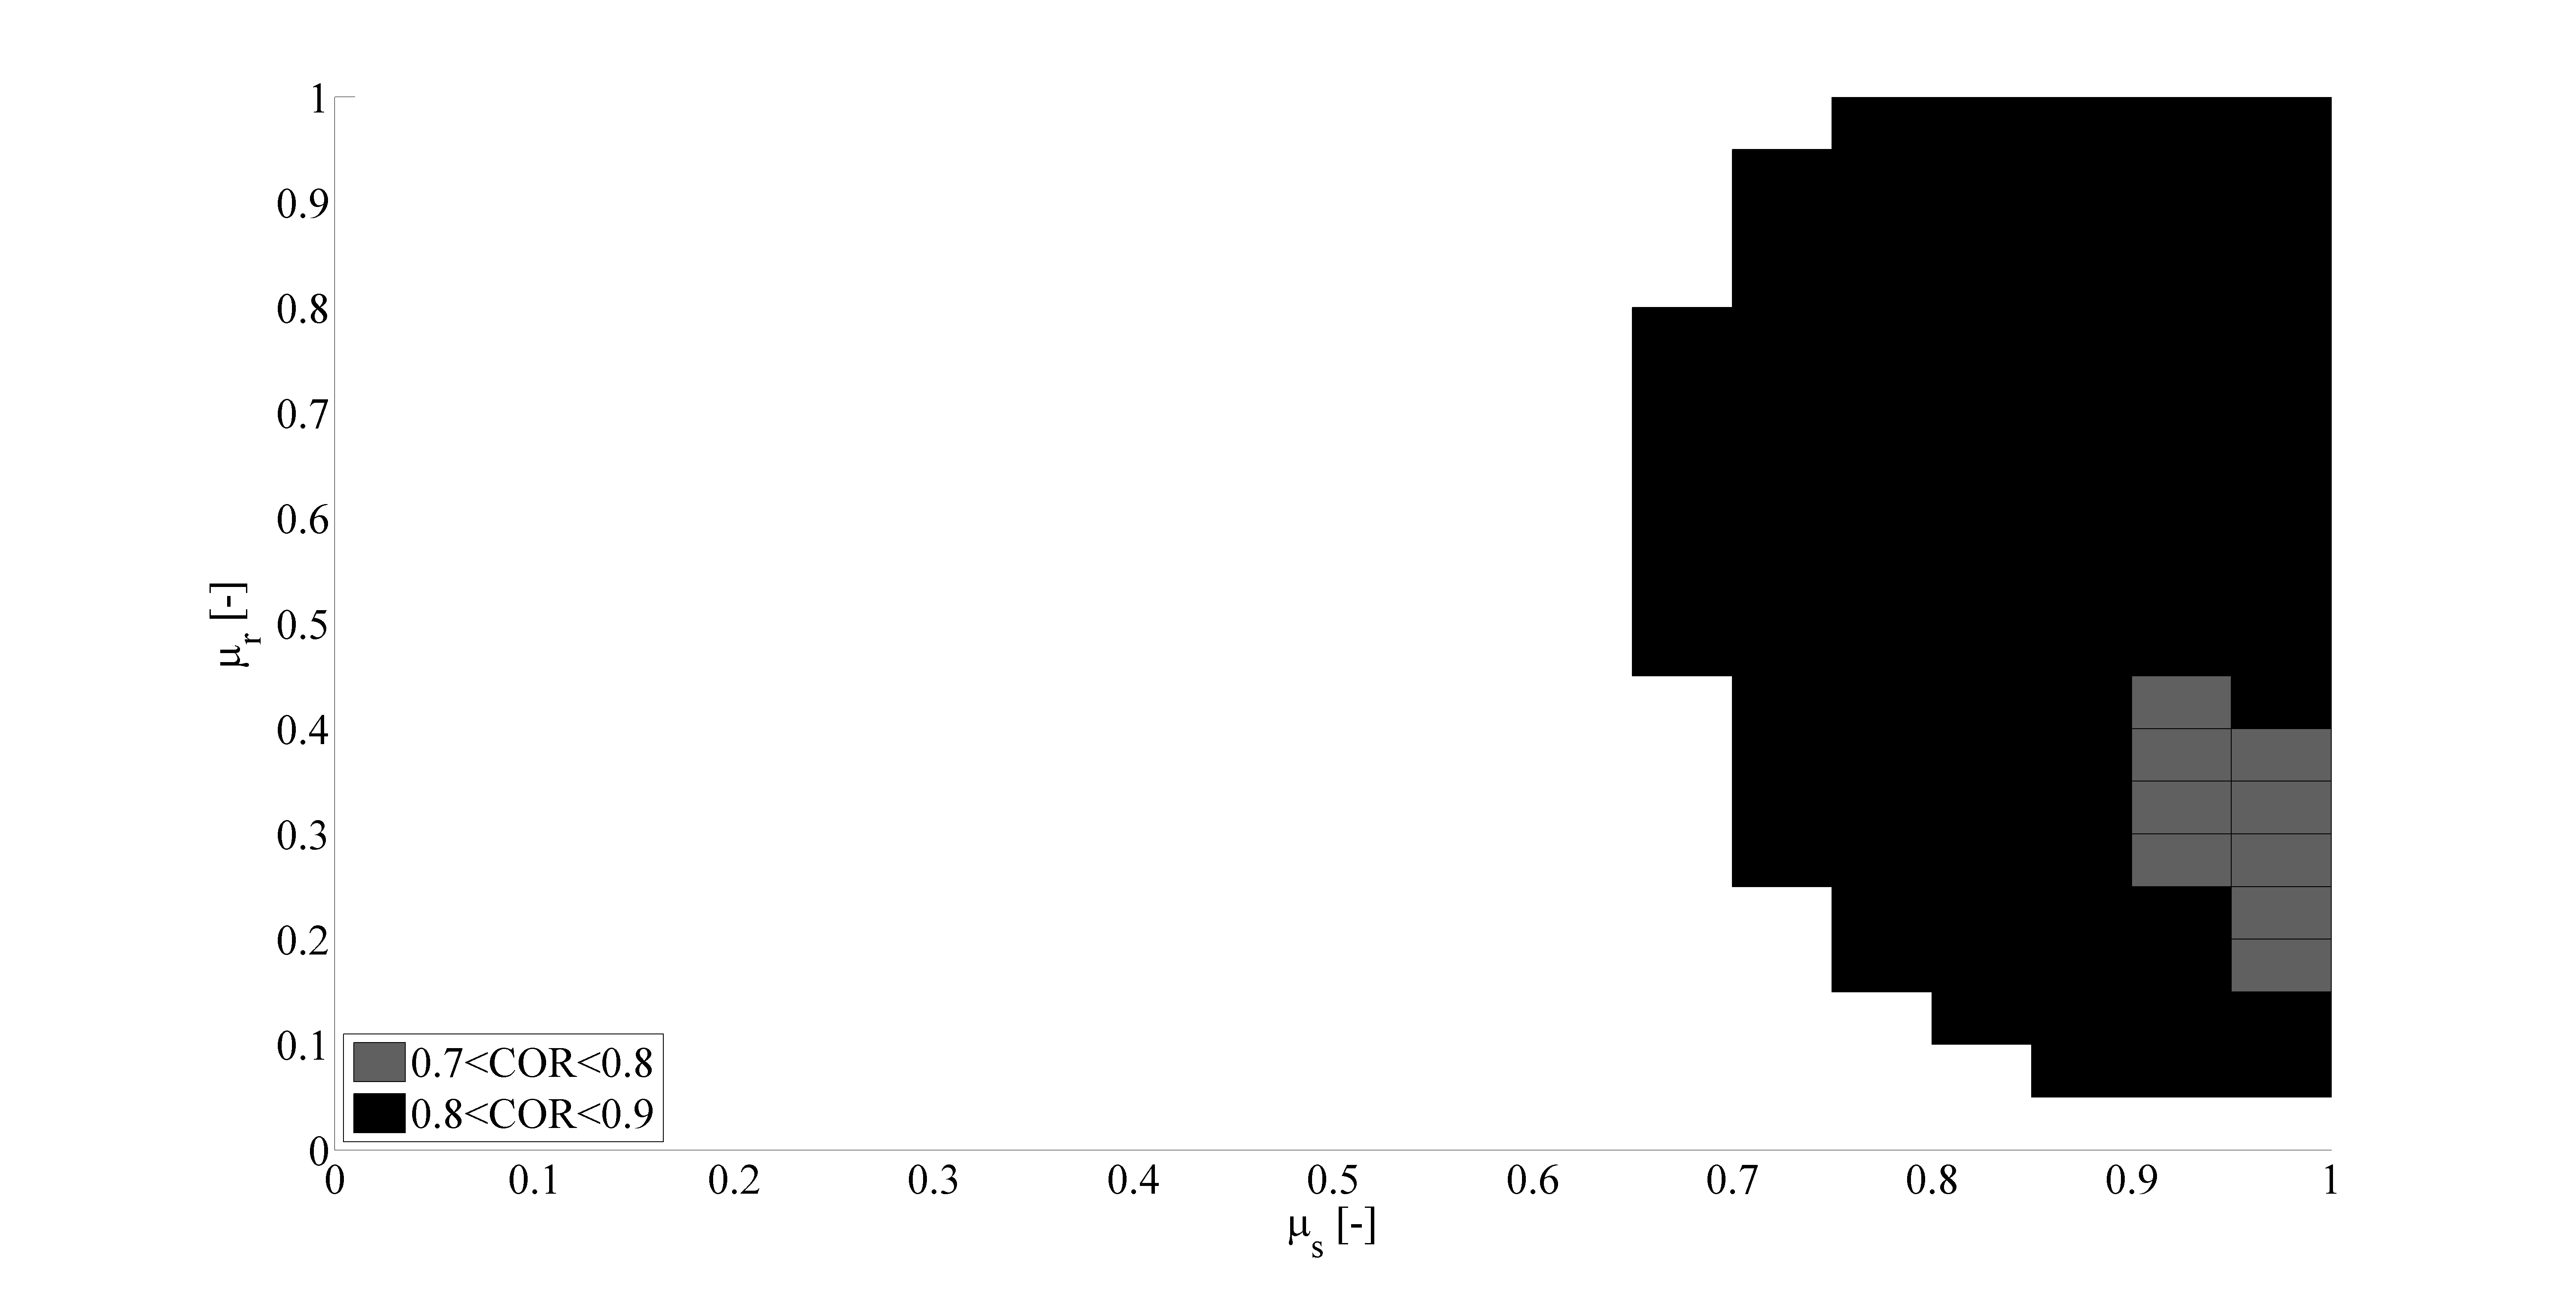
\includegraphics[width=.48\columnwidth]{images/30cloudpirker12schulze10070} 
\caption{Density plot, $SSC$, $\sigma_n=10070$ Pa, P=1.2}
\label{fig:30cloudpirker12schulze10070} 
\end{figure}
%************************************************

\begin{figure}%[!htb] 
\centering 
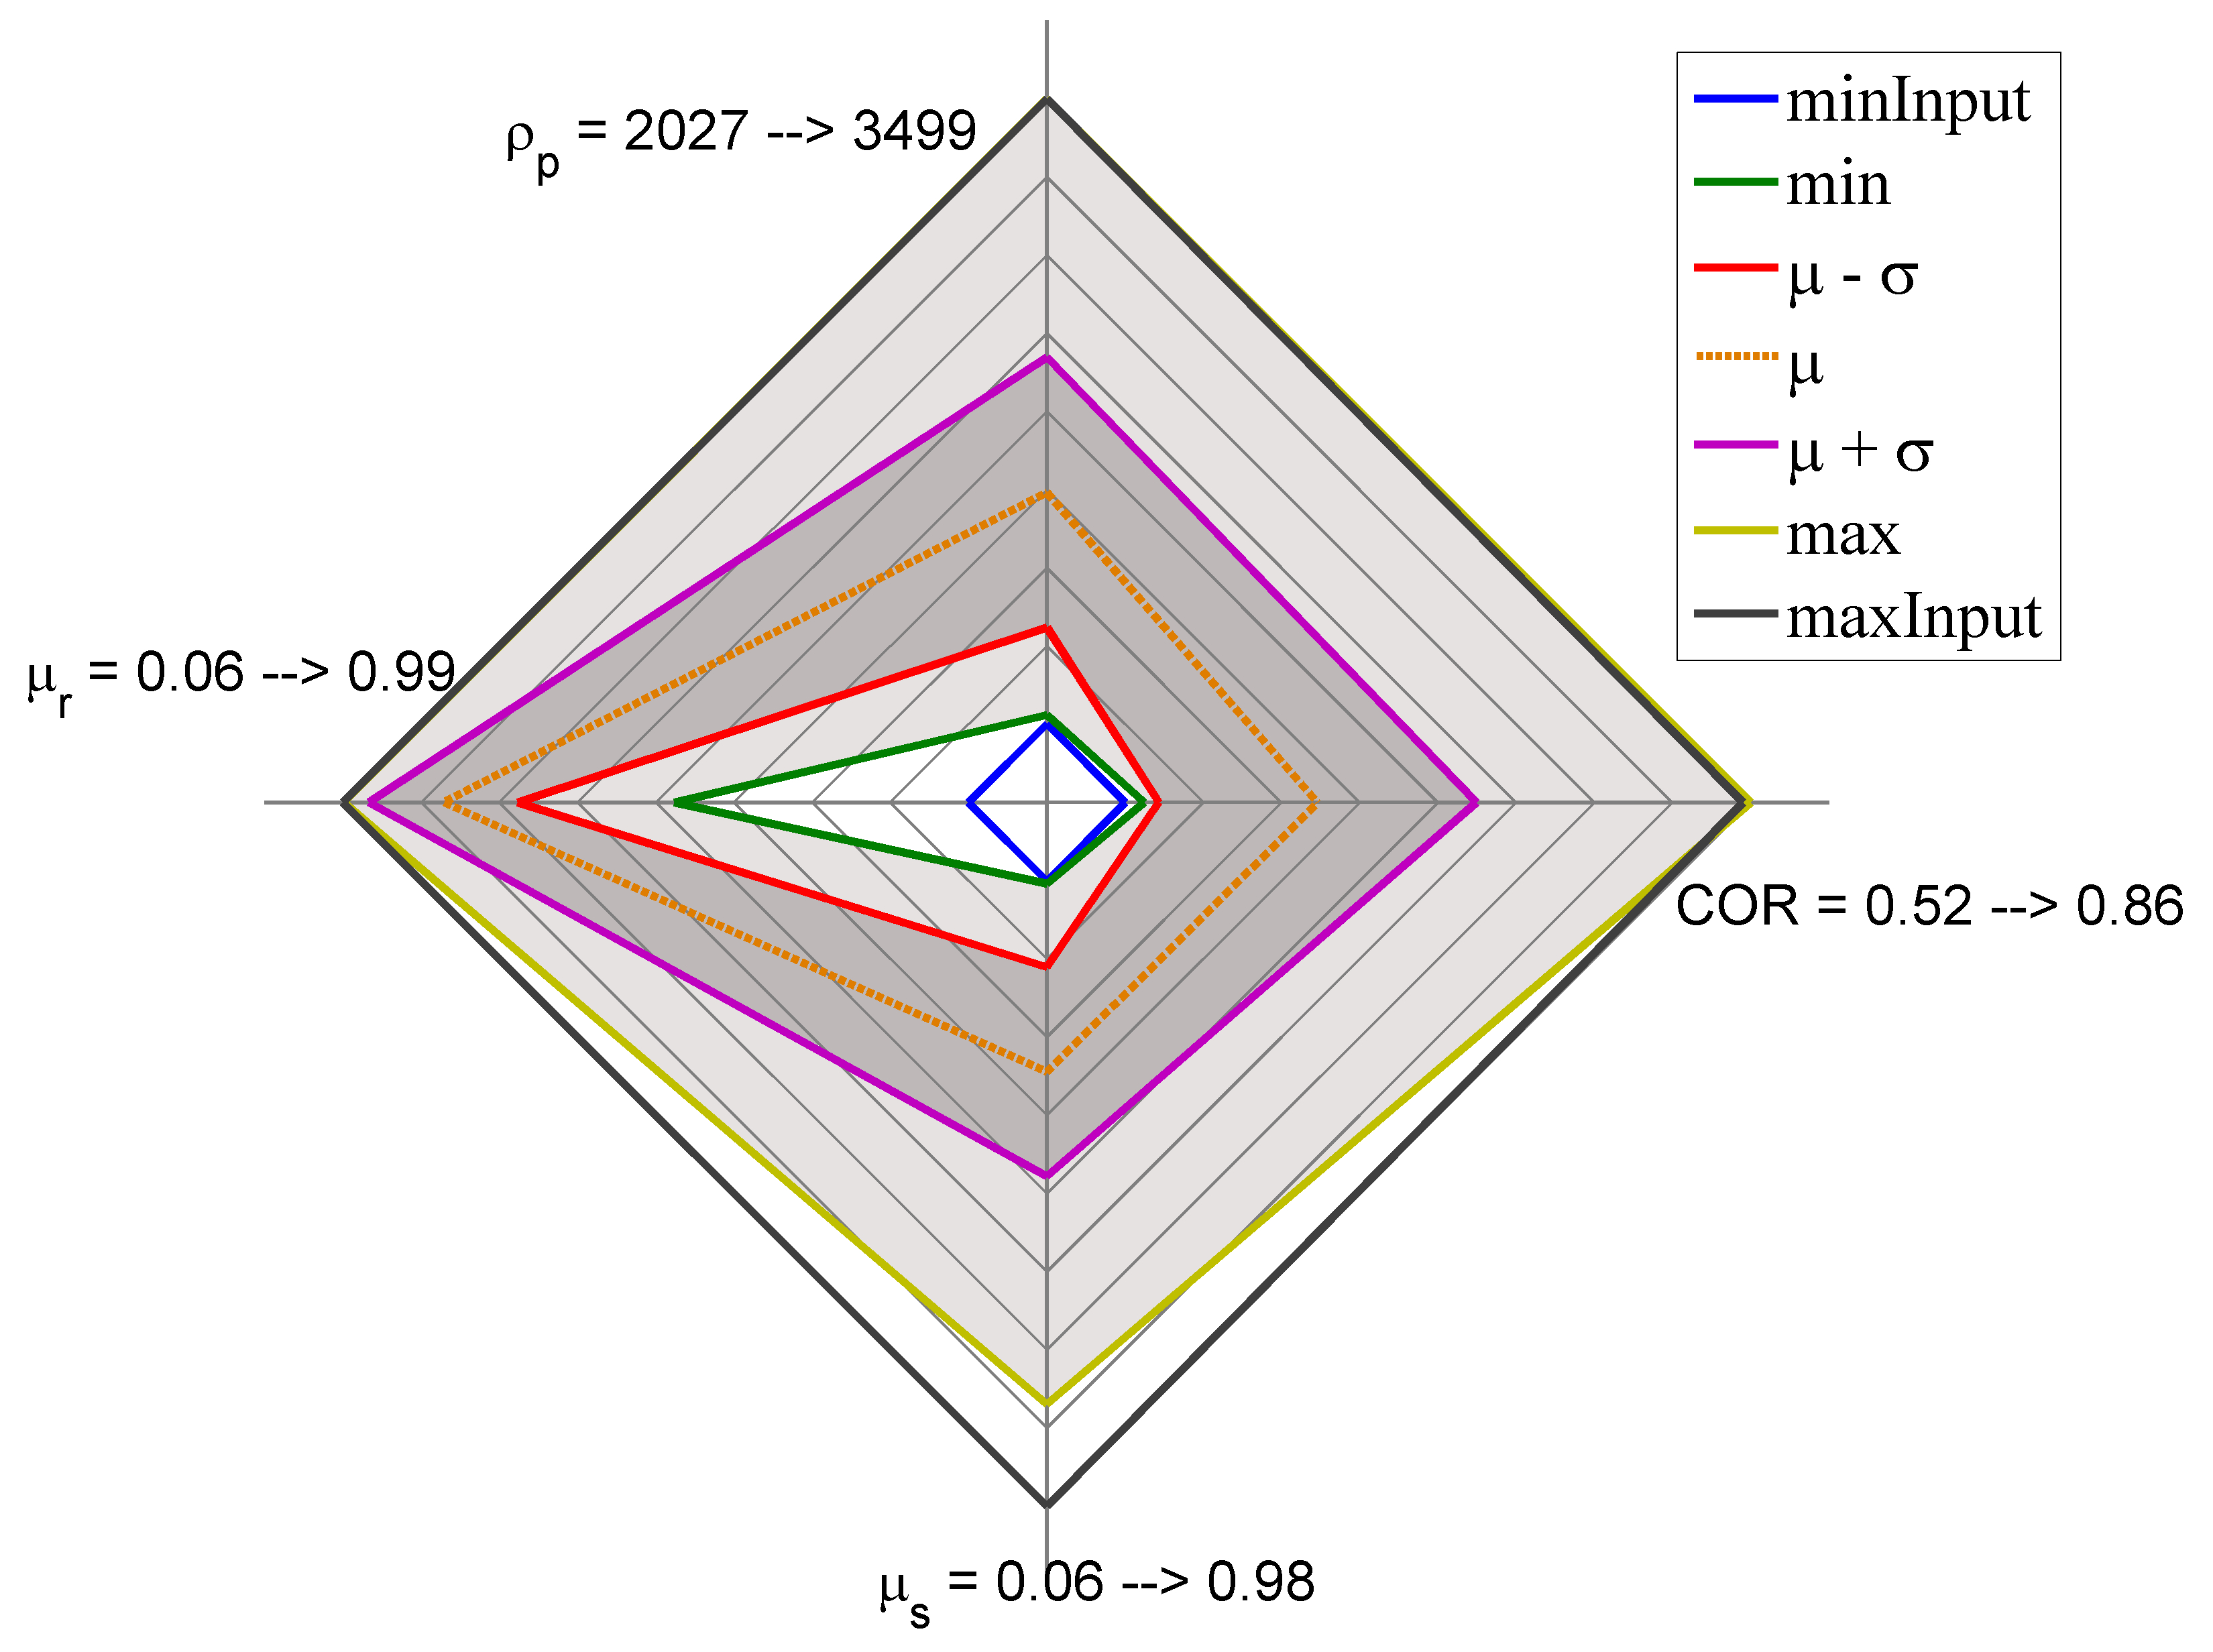
\includegraphics[width=.48\columnwidth]{images/31radarpirker1aor} 
\caption{Parameter space plot, $AoR_{exp} = 38.85 ^\circ$}
\label{fig:31radarpirker1aor} 
\end{figure}
%************************************************
\begin{figure}%[!htb] 
\centering 
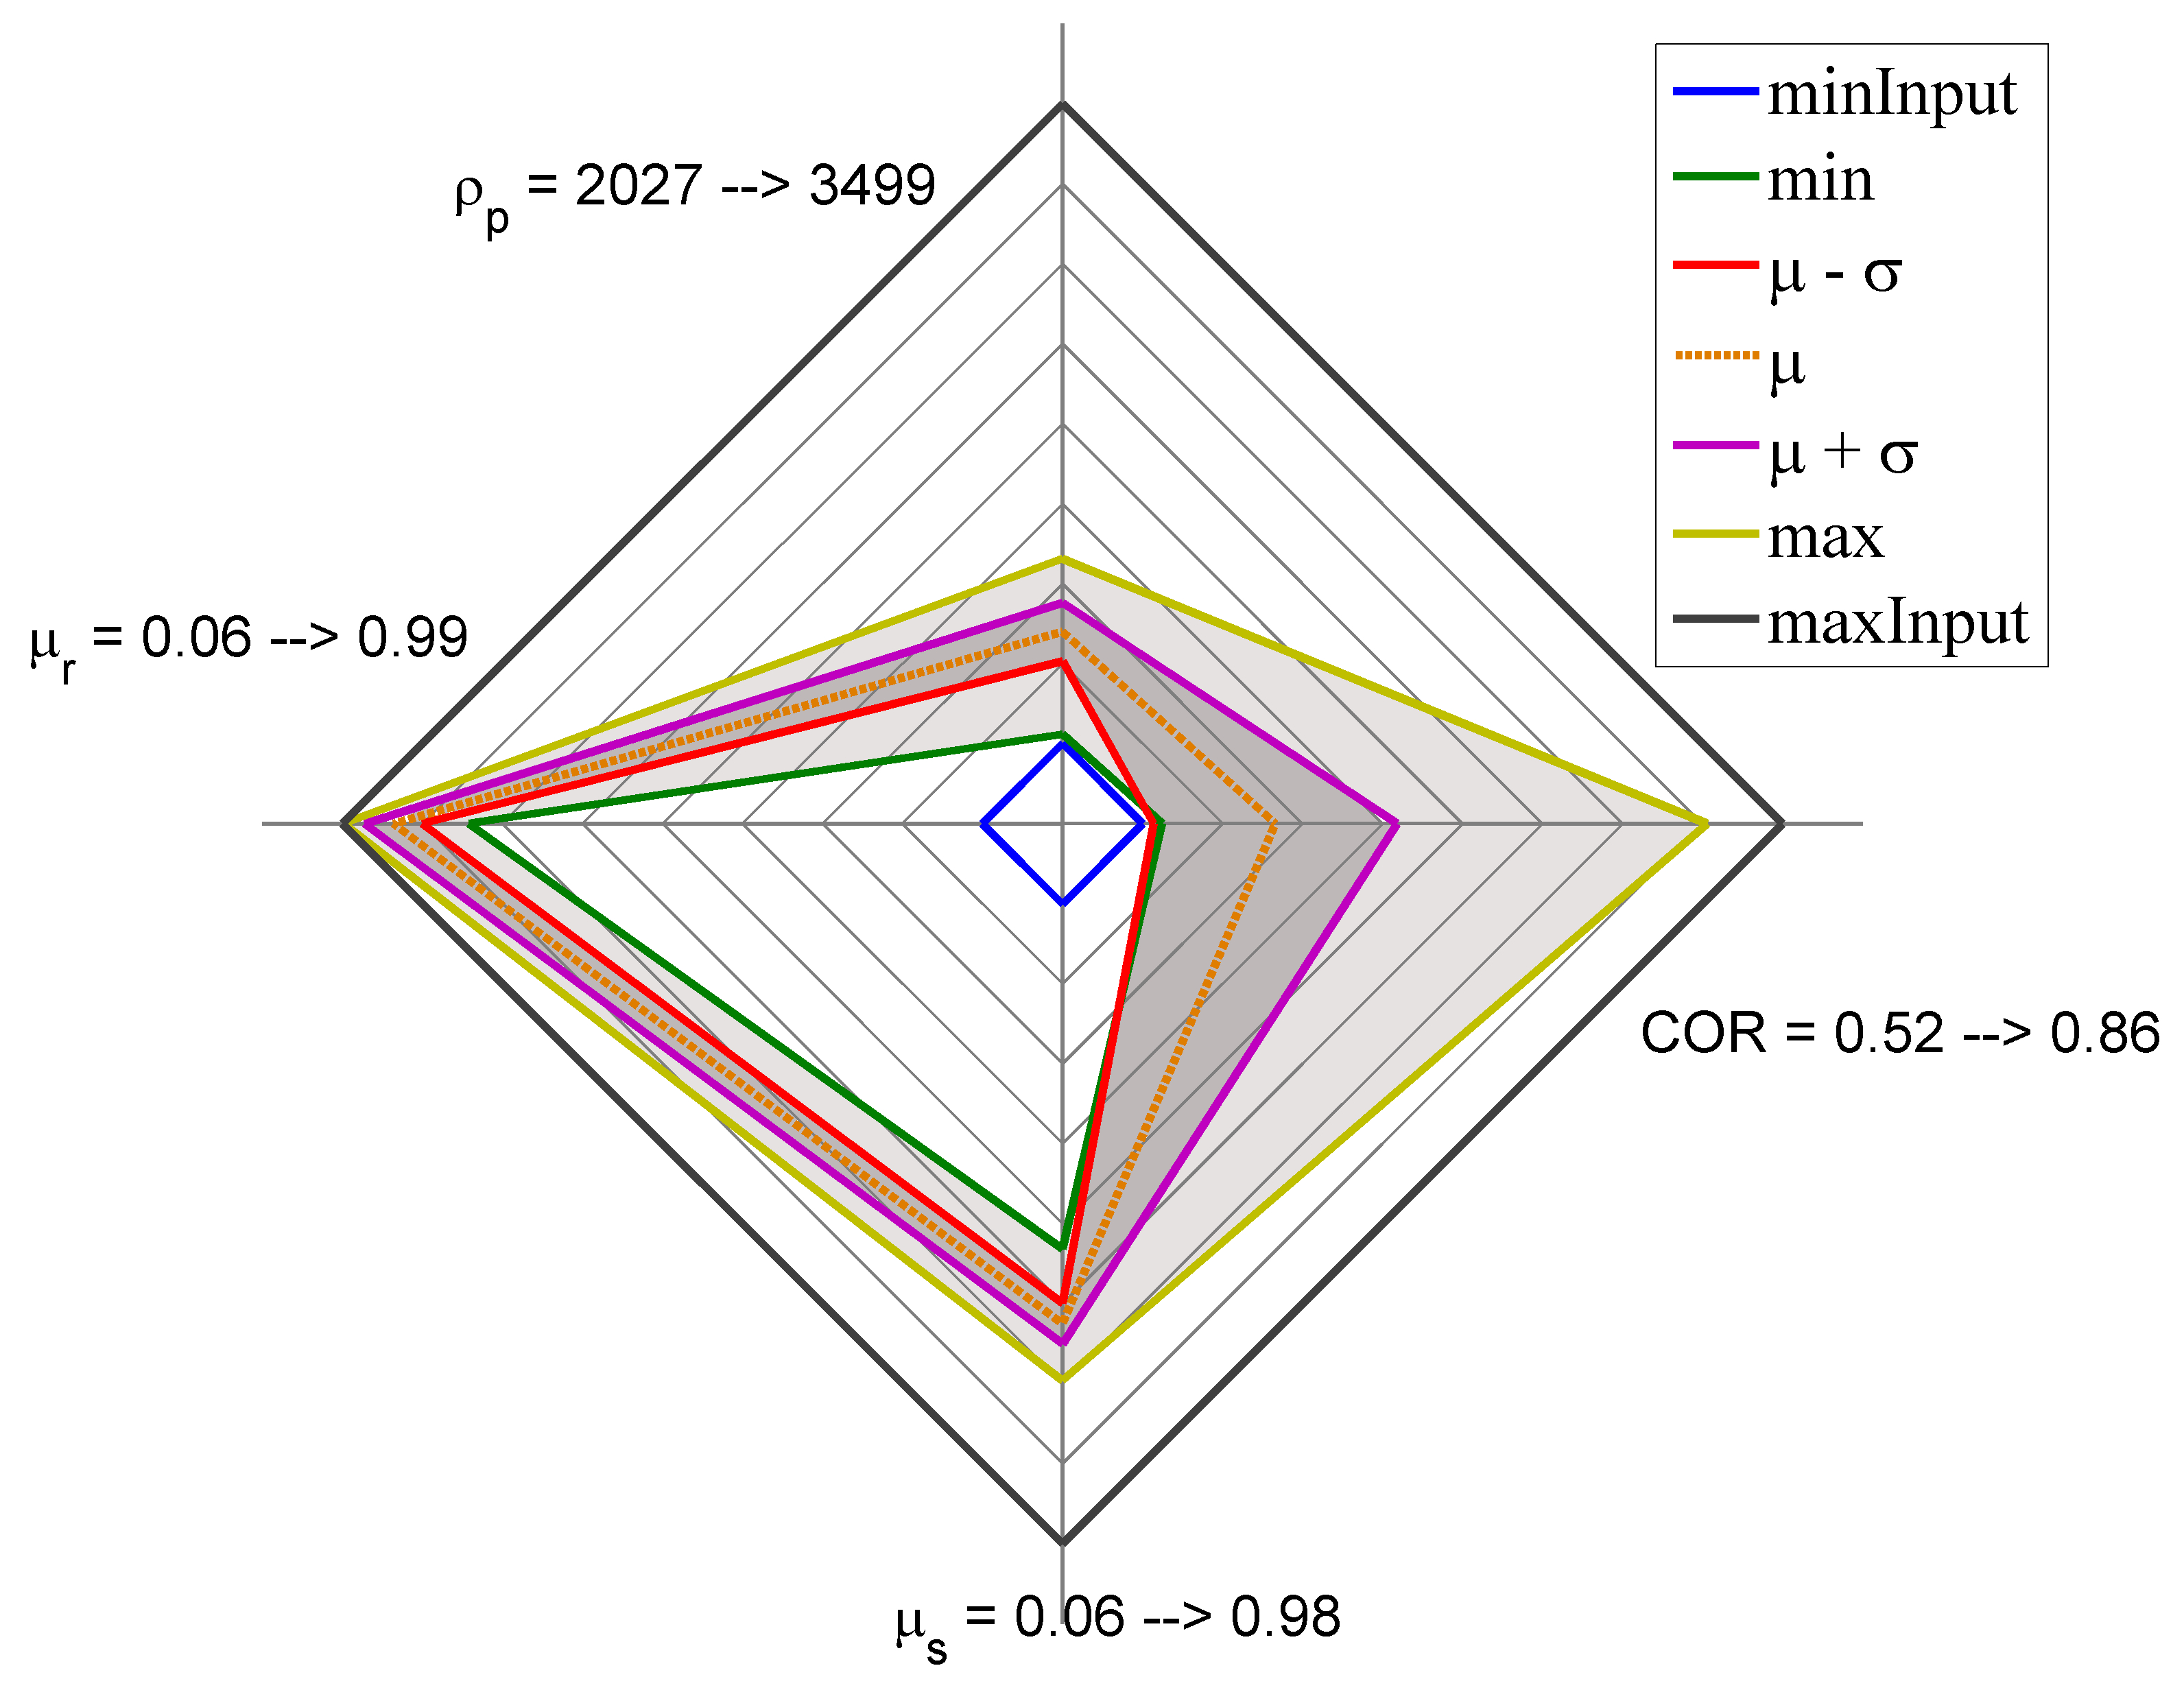
\includegraphics[width=.48\columnwidth]{images/33radarpirker1schulze10070aor} 
\caption{Parameter space plot, $AoR_{exp} = 38.85
        ^\circ$ \& $SSC$: $\sigma_n=10070$ Pa}
\label{fig:33radarpirker1schulze10070aor} 
\end{figure}
%************************************************